\documentclass[12pt]{article}
%\usepackage{jmlda}
\usepackage{cmap}
\usepackage[T2A]{fontenc}
\usepackage[utf8]{inputenc}
\usepackage{amsmath,amssymb,mathrsfs,mathtext}
\usepackage[russian]{babel}
\usepackage{graphicx}
\usepackage{enumerate}
\usepackage{fancyhdr}
\usepackage{a4wide}
\usepackage{cite}
%\renewcommand{\headrulewidth}{0pt}
\DeclareMathOperator*{\argmin}{arg\,min}
\DeclareMathOperator*{\argmax}{arg\,max}
\begin{document}
\title{Глубокое обучение в задачах классификации временных рядов%Глубокое обучение  в задаче распознавания временных рядов с использованием графического процессора и облачного сервиса
}
\date{}
\maketitle

 \begin{center}
 {О.\,Ю.~Бахтеев \\ {Московский физико-технический институт, bakhteev@phystech.edu},
 \\ М.\,С.~Попова \\ {Московский физико-технический институт, maria\_popova@phystech.edu},
 \\ В.\,В.~Стрижов \\ {Вычислительный центр им. А.~А. Дородницына
 ФИЦ ИУ РАН% Федерального исследовательского центра <<Информатика и управление>> Российской академии наук
, strijov@ccas.ru}} % основной список авторов, выводимый в оглавление
 \end{center}


\bigskip
\textbf{Ключевые слова}:  классификация временных рядов; глубокое обучение; суперпозиция моделей; автокодировщик; ограниченная машина Больцмана; Theano; Amazon Web Services

Решается задача классификации временных рядов акселерометра мобильного телефона. Строится сеть глубокого обучения. Структура сети --- композиция ограниченной машины Больцмана, автокодировщика и двухслойной нейросети. Анализируется зависимость ошибки классификации от числа параметров и размера обучающей выборки.  Работа посвящена построению сети глубокого обучения и оптимизации ее параметров с помощью вычислительных мощностей графического ускорителя на основе сервиса облачных вычислений Amazon Web Services.  

Эксперимент проводится с использованием Theano --- библиотеки для вычислений для языка Python. Theano активно используется для построения моделей глубокого обучения, а также для построения более специализированных библиотек. Функции вычислений Theano компилируются, что позволяет выполнять вычисления за приемлемое время. Другой отличительной особенностью Theano является возможность применения графического процессора с использованием архитектуры параллельных вычислений CUDA. Также в экспериментальном режиме доступна возможность применить интерфейс OpenCL.

\paragraph{Формальная постановка задачи}
Пусть задана выборка \begin{equation}\label{eq:dataset}\mathfrak{D} = \{(\mathbf{x}_i,y_i)\}, i = 1,\dots,N,\end{equation} состоящая из множества пар <<объект -- класс>>, $\mathbf{x}_i \in \mathbb{R}^n$. Каждый объект $\mathbf{x}$ принадлежит одному из $Z$ классов с меткой $y_i \in \mathbf{Y} = \{1,\dots,Z\}$.

Моделью классификации или сетью глубокого обучения $\mathbf{f}$ назовем суперпозицию функций
\begin{equation}
\label{eq:main}
 \mathbf{f}(\mathbf{w}, \mathbf{x}) = \boldsymbol{{\mu}}_3(\boldsymbol{\mu}_2( \boldsymbol{\mu}_1(\mathbf{x}))): \mathbb{R}^n \to [0,1]^Z,
\end{equation}
где $\boldsymbol{\mu}_k, k \in \{1,\dots,3\},$ --- модели, параметрическое семейство вектор-функции; $\mathbf{w}$ --- вектор параметров моделей;
$r$-ю компоненту вектора $\mathbf{f}(\mathbf{x},\mathbf{w})$ будем интерпретировать как вероятность отнесения объекта $\mathbf{x}_i$ к классу с меткой $r$.

Требуется минимизировать функцию ошибки $S$ на обучающей выборке $\mathfrak{D}$:
\[
 \hat{\mathbf{w}} = \argmin_\mathbf{w} S(\mathbf{w}|\mathfrak{D}),
\]
где $S$ --- сумма отрицательных логарифмов правдоподобия по всем объектам выборки:
\[
 S(\mathbf{w}|\mathfrak{D}) = -\sum_{(\mathbf{x},y) \in \mathfrak{D} } \sum_{r=1}^Z [y_i = r] \text{log} p(y=r|\mathbf{x},\mathbf{w}).
\]
Сеть глубокого обучения состоит из трех основных компонент:
ограниченной машины Больцмана~$\boldsymbol{\mu}_1$, автокодировщика~$\boldsymbol{\mu}_2$ и двухслойной нейросети с softmax-классификатором~$\boldsymbol{\mu}_3$.


\paragraph{Общий план запуска алгоритма.}
Для запуска алгоритма на сервере AWS требуется зарегистрироваться на AWS, сконфигурировать экземпляр AWS (instance), скопировать код и данные проекта на сервер и подключиться к серверу по протоколу SSH. После этого требуется зайти в папку с проектом, запустить вычислительный эксперимент, скопировать полученные результаты эксперимента на локальный компьютер и уничтожить экземпляр.

\paragraph{Вычислительный эксперимент}
Набор данных содержит записи движений для 6 классов переменной длины по трем координатам  акселерометра мобильного телефона. Из каждой записи использовались первые 200 сегментов. Пример данных из выборки WISDM приведен на рис.~\ref{fig:wisdm}. Т. к. выборка не сбалансирована, в нее добавлялись повторы записей классов, содержащих количество записей, меньшее чем у большего класса.

\begin{figure}[tb!]
 \centering
  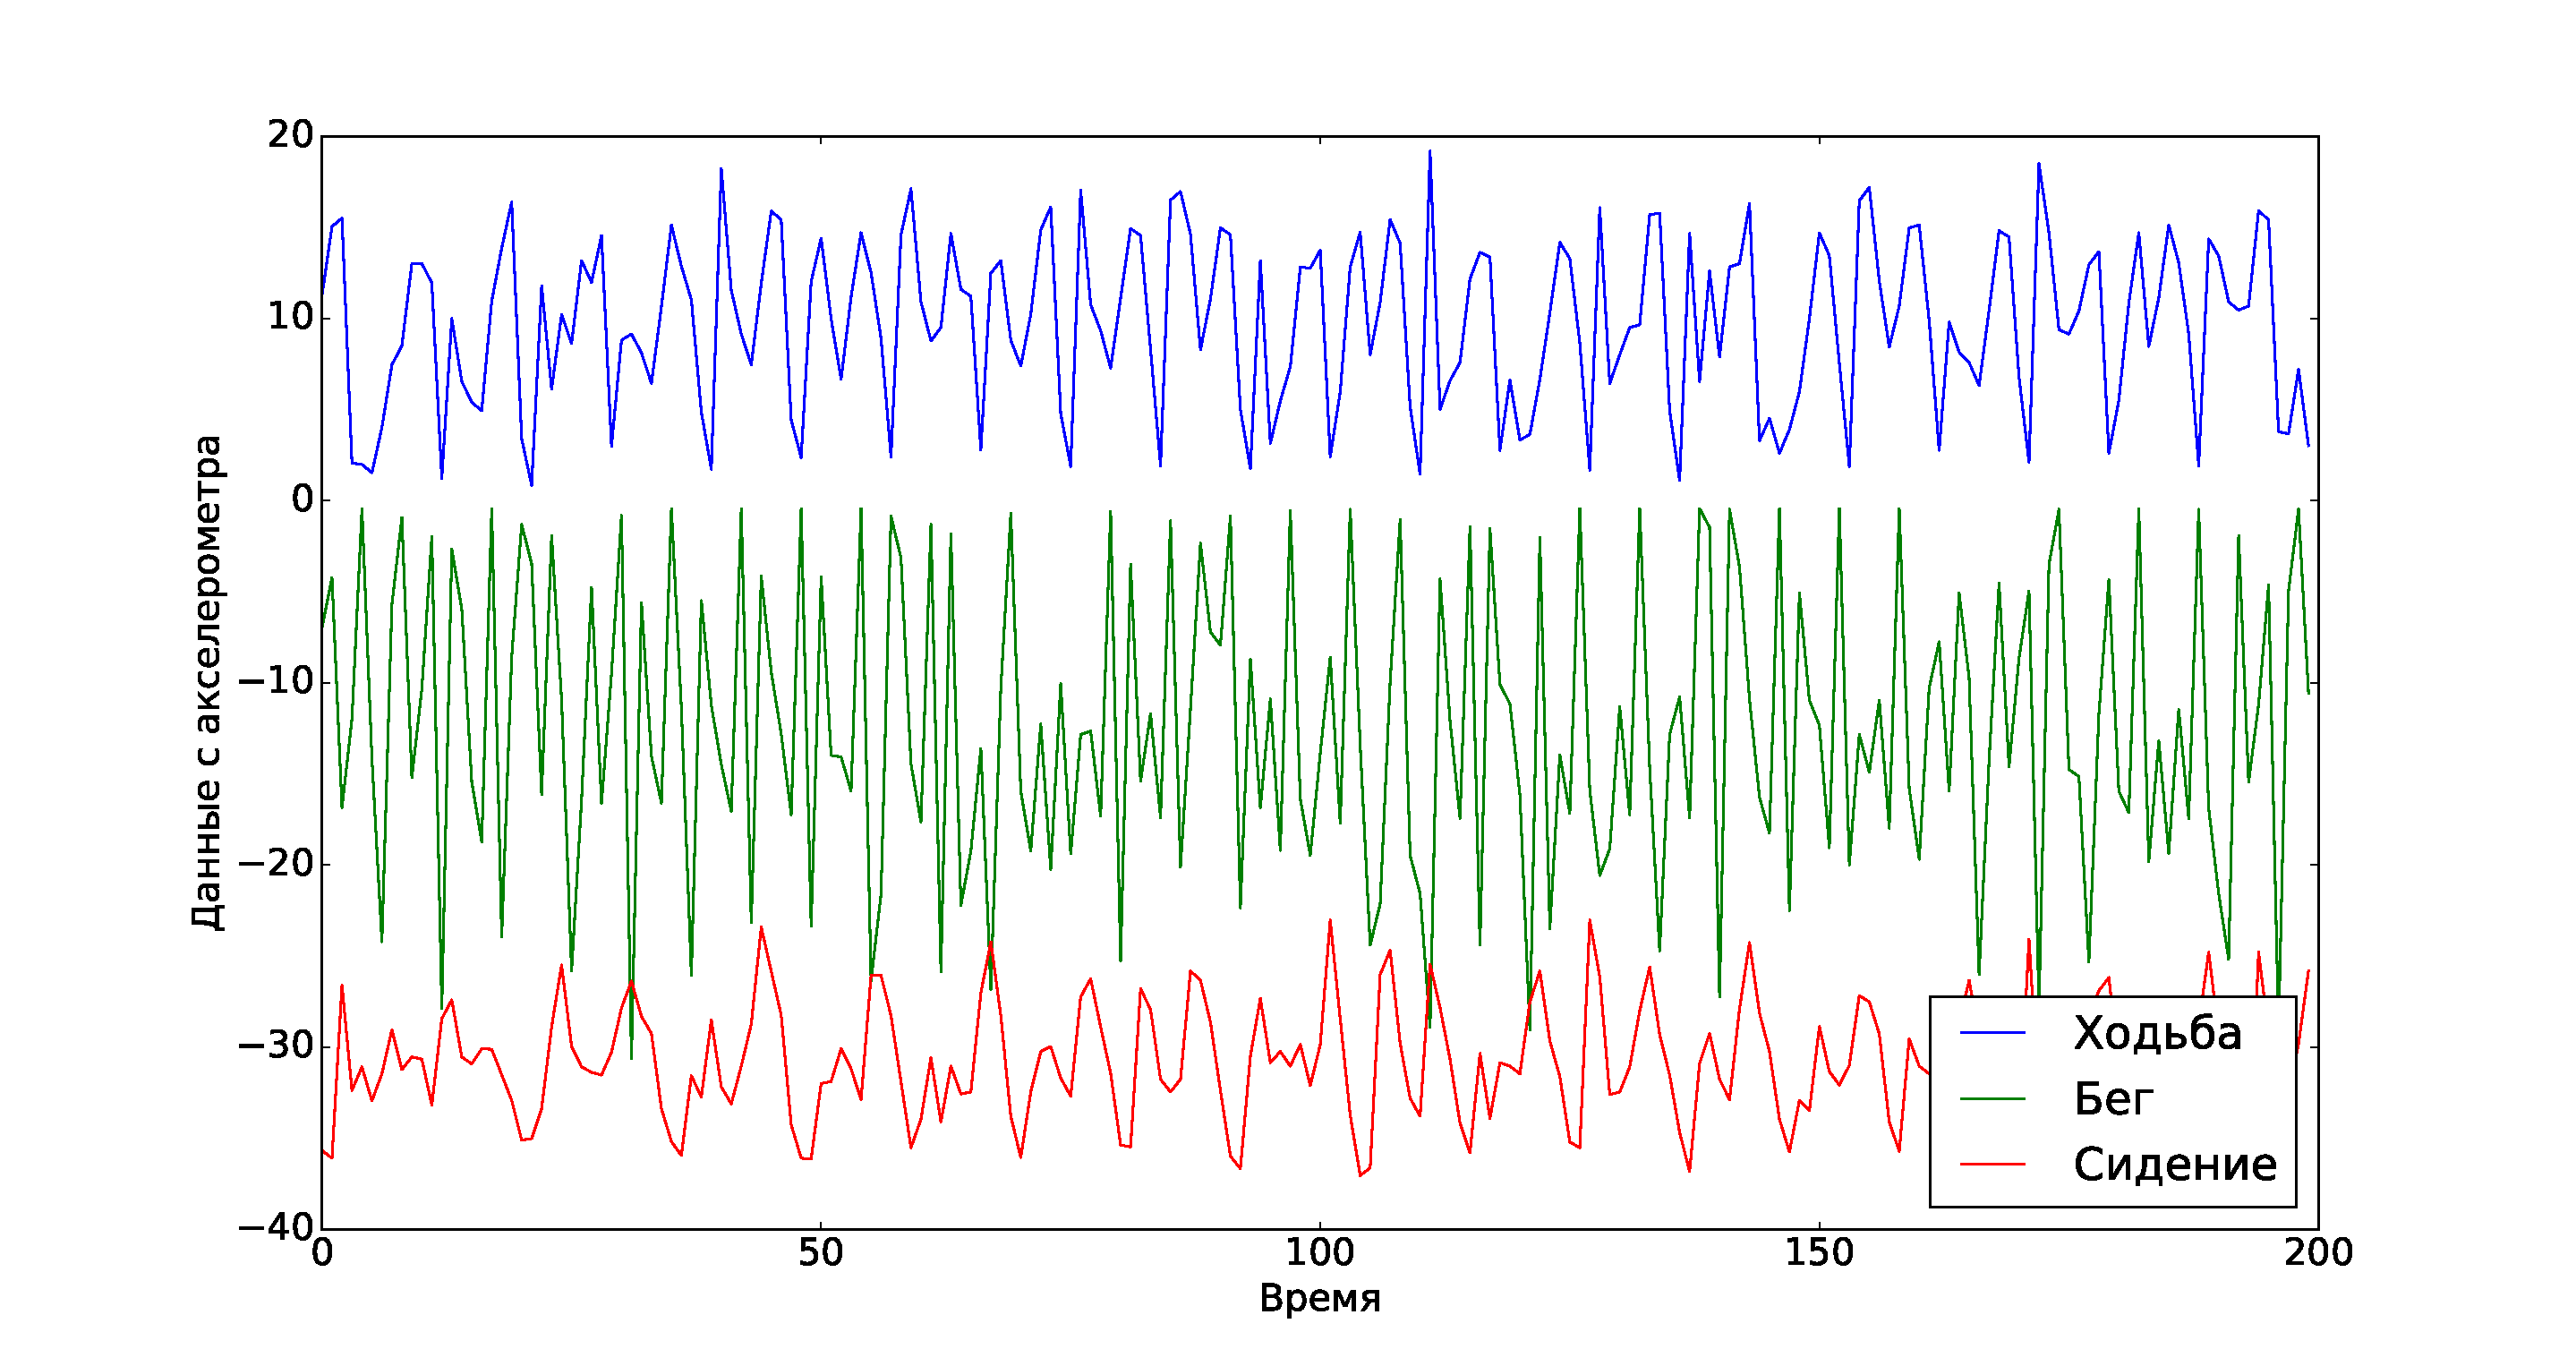
\includegraphics[width=1.0\textwidth]{wisdm.pdf}
 \caption{Пример временных рядов из выборки WISDM, проекция на первую координату. Проекции, соответствующие сидению и бегу были сдвинуты для наглядности.}
 \label{fig:wisdm}
\end{figure}


\begin{figure}[tb!]
 \centering
  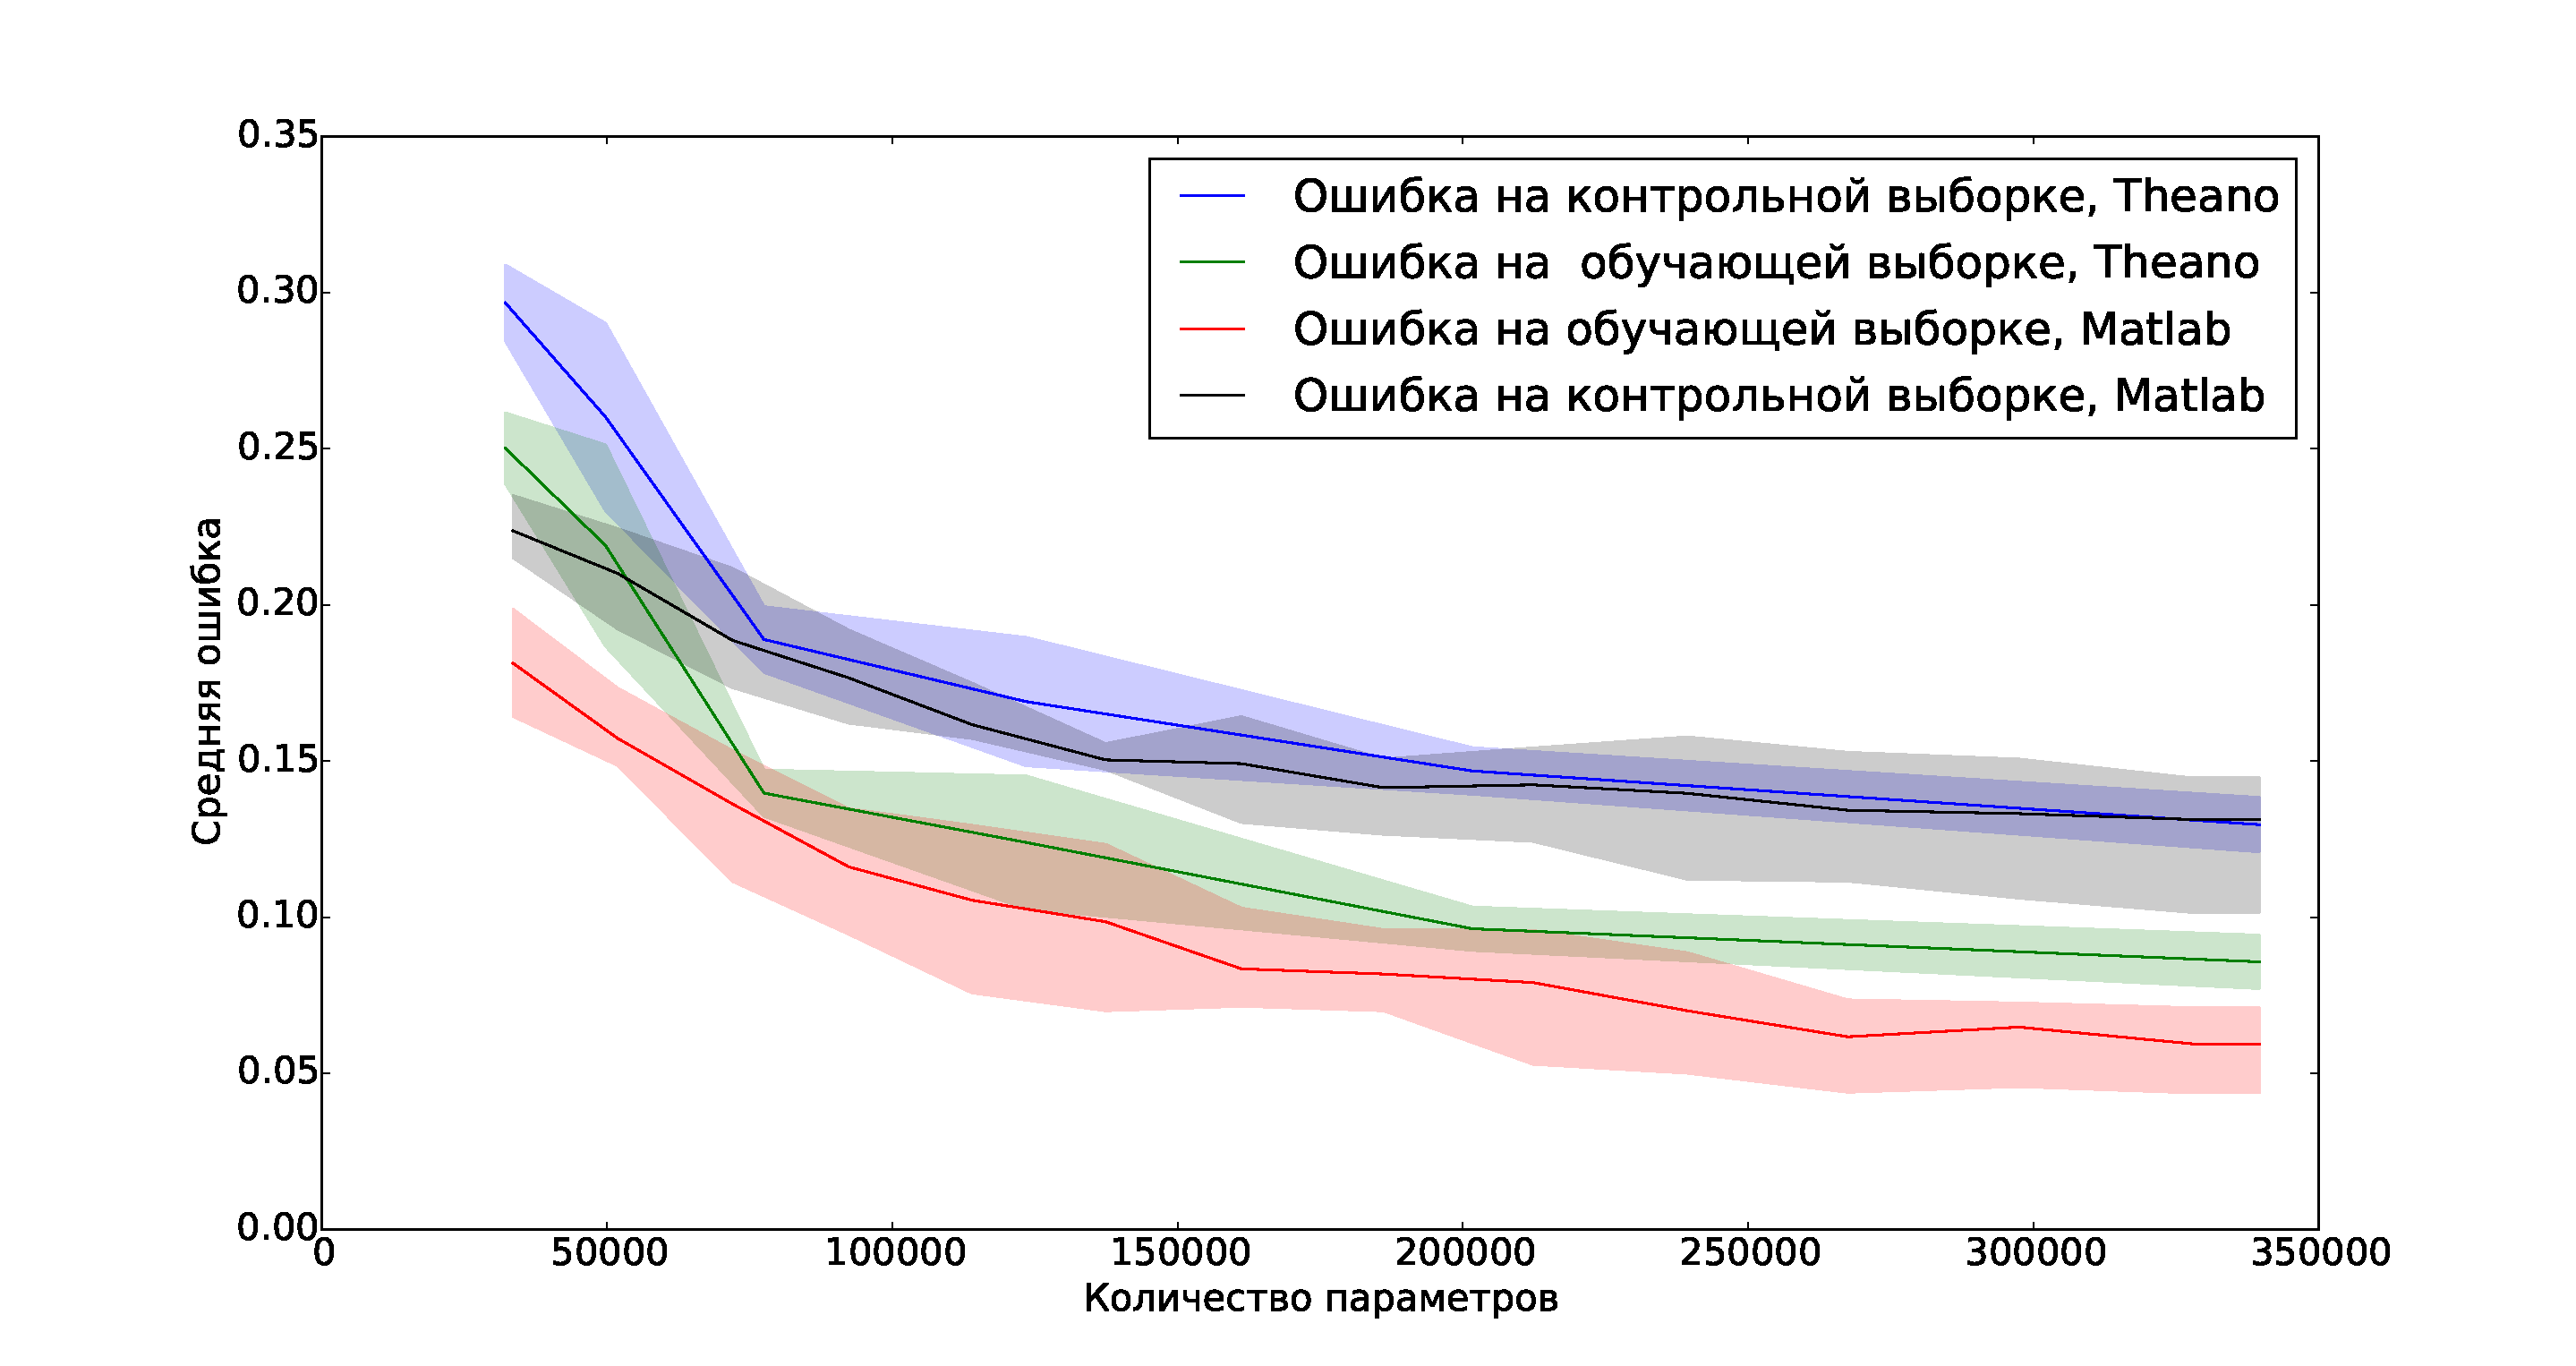
\includegraphics[width=1.0\textwidth]{neurons.pdf}
 \caption{Зависимость ошибки от числа нейронов}
 \label{fig:neurons}
\end{figure}


Для оценки зависимости качества классификации от размера обучающей выборки была проведена кроссвалидация с фиксированным количеством объектов в обучающей выборке (25\% исходной выборки) и переменным размером обучающей выборки. Число нейронов было установлено как 364:224:112. При проведении процедуры скользящего контроля для каждого отсчета было произведено пять запусков. График зависимости ошибки классификации от размера обучающей выборки представлен на рис.~\ref{fig:samples}.


\begin{figure}[tb!]
 \centering
  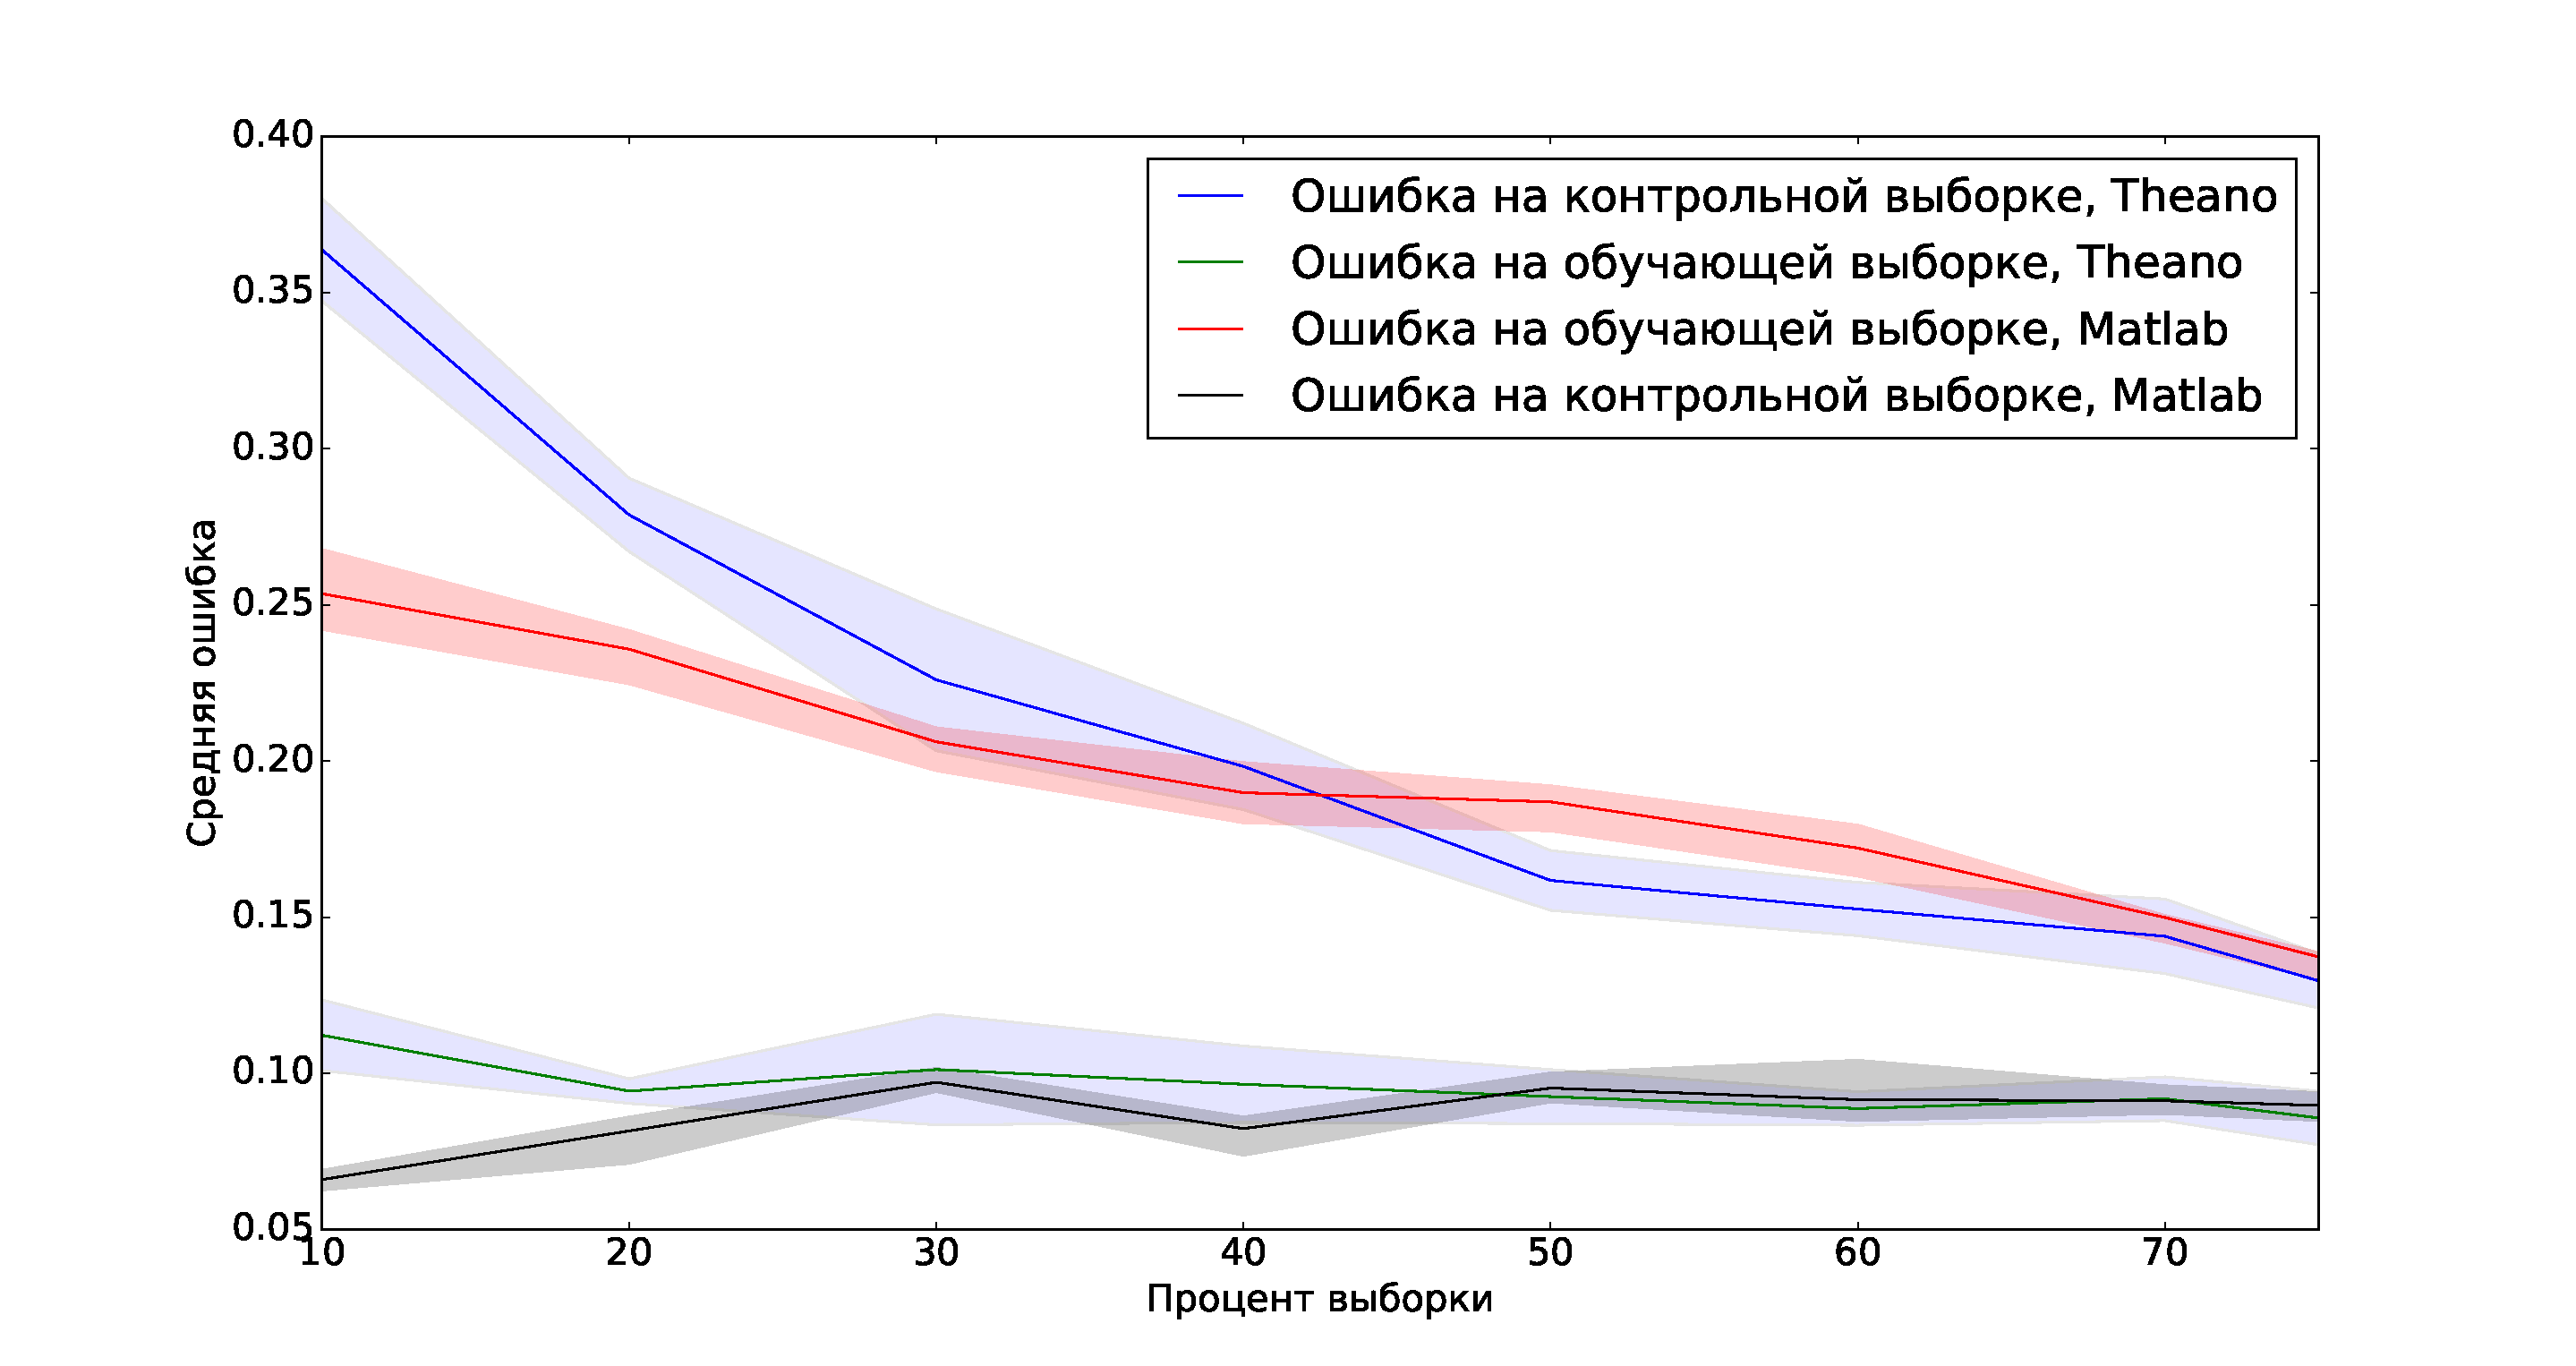
\includegraphics[width=1.0\textwidth]{samples.pdf}
 \caption{Зависимость ошибки от размера обучающей выборки}
 \label{fig:samples}
\end{figure}


Для исследования скорости работы процесса обучения нейросети в зависимости от конфигурации Theano был сделан следующий эксперимент:
проводилось обучение двухслойной нейросети на основе подсчитанных заранее параметров ограниченной машины Больцмана и автокодировщика. Обучение проходило за 100 итераций. При обучении алгоритм запускался параллельно с $n$ разными стартовыми позициями, $n \in \{1,\dots,4\}.$ Число нейронов было установлено как 300:200:100.
Запуск осуществлялся со следующими конфигурациями Theano:
\begin{itemize}
\item вычисление на центральном процессоре, задействовано
одно ядро;
\item вычисление на центральном процессоре, задействовано четыре ядра;
\item вычисление на центральном процессоре, задействовано восемь ядер;
\item вычисление на графическом процессоре.
\end{itemize}

Результаты эксперимента приведены на рис.~\ref{fig:speed}. Как видно из графика, вычисление с использованием CUDA показывает значительное ускорение по сравнению с вычислением на центральном процессоре. Детальное описание структуры нейросети можно найти в статье \emph{Бахтеев О. Ю., Попова М.С., Стрижов В.В. } Системы и средства глубокого обучения в задачах классификации // Системы и средства информатики. — 2016. — № 2.


\begin{figure}[tb!]
 \centering
  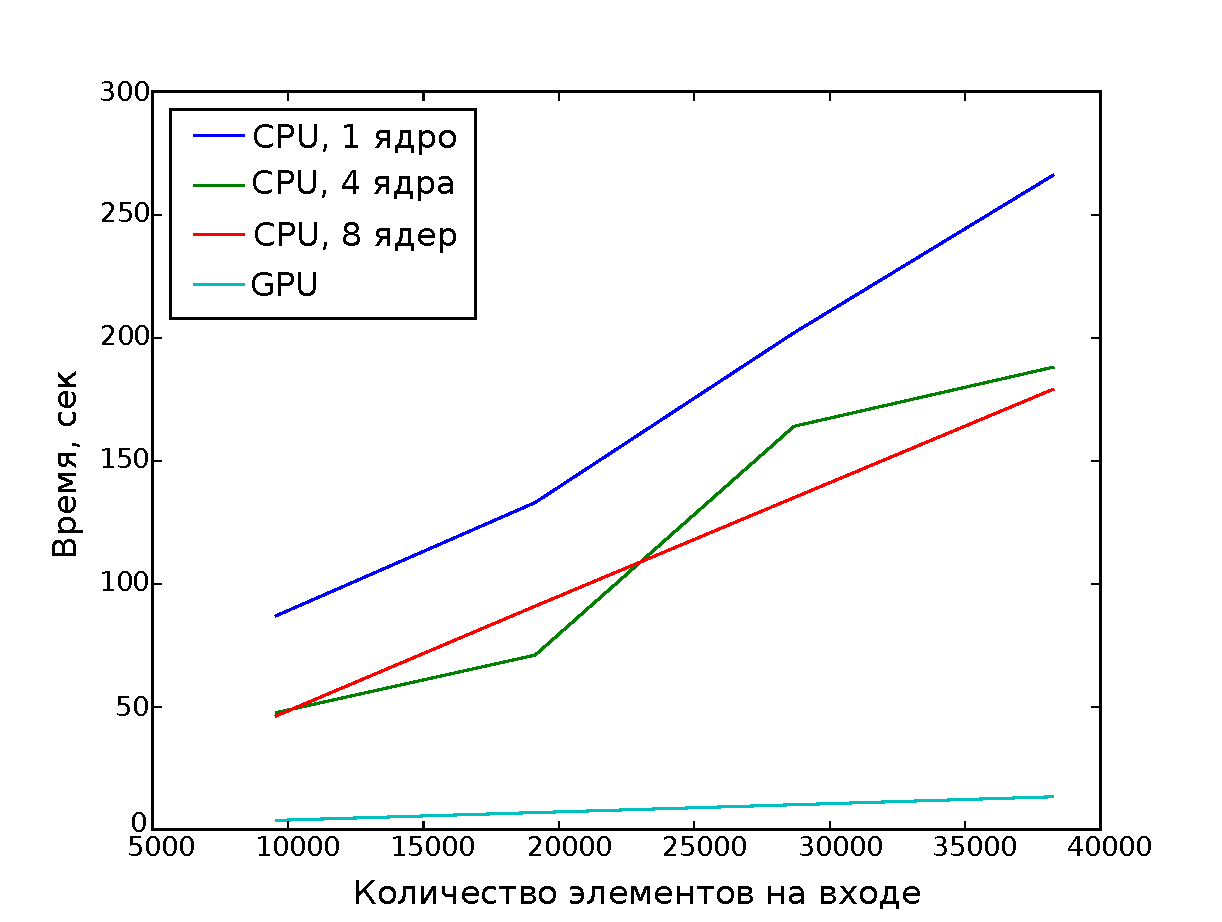
\includegraphics[width=0.8\textwidth]{result.pdf}
 \caption{Результаты эксперимента по исследованию скорости процесса обучения}
 \label{fig:speed}
\end{figure}

\end{document}
